\documentclass[a4paper,11pt]{article}

%% Language and font encodings
\usepackage[spanish,es-tabla]{babel}
\usepackage[utf8x]{inputenc}
%\usepackage{natbib}
\usepackage{booktabs}
\usepackage{tabu}
\usepackage[T1]{fontenc}
\usepackage{subcaption}
\usepackage{float}
\usepackage{amssymb}
\usepackage{multirow}
\usepackage{comment}
\usepackage{times} % pára el tipo de letra arial
\usepackage{wrapfig}
\usepackage{lscape}
\usepackage{cite}
%% Sets page size and margins
\usepackage[a4paper,top=1.8cm,bottom=1.8cm,left=1.5cm,right=1.5cm,marginparwidth=1.75cm]{geometry}

%% Useful packages
\usepackage{amsmath}
\usepackage{graphicx}
%\usepackage{apacite}
\usepackage[colorinlistoftodos]{todonotes}
\usepackage[colorlinks=true, allcolors=blue]{hyperref}

\renewcommand{\labelenumii}{\theenumii}
\renewcommand{\theenumii}{\theenumi.\arabic{enumii}.}

\title{ 
	
	NeoArgos-tools: Un \textit{Pipeline} de Detección \textit{In-silico} de Neoantígenos de Cáncer para el Desarrollo de Vacunas Personalizadas
}

%\title{Desarrollo de una Aplicación Web para la Detección de Neoantígenos en el Marco de Desarrollo %de Vacunas Personalizadas para Tratar el Cáncer }
%\author{Vicente Machaca  e Yván Túpac}
\author{}
%\date{\today}
\date{}

\begin{document}
	

	
	
	
	
	
	
	
	%\maketitle

\part*{Propuesta de la Investigación}

\section{Título}
Desarrollo de una herramienta  para la detección \textit{in silico} de neoantígenos a partir de datos genómicos en el marco de desarrollo de vacunas personalizadas para tratar el cáncer.

\section{Resumen (5K)}
La detección de neoantígenos es una área de la Bioinformática la cual es de suma importancia debido a su aplicabilidad para el desarrollo de vacunas personalizadas contra el cáncer. Estas vacunas en conjunto con otros tratamientos como radioterapias y quimioterapias han presentado resultados prominentes. En este contexto, en este proyecto se determina el desarrollo de un pipeline para la detección de neoantígenos. La herramienta nombrada es NeoArgosTools v2.0. La herramienta tomará como entrada datos genómicos como RNA-seq/DNA-seq y datos de Mass Spectrometry. Luego, va a integrar herramientas de alineamiento de secuencias, detección de variaciones estructurales/fusión de genes, llamado de variantes, y anotación de variantes para obtener los neoantígenos candidatos y los tipos de proteínas Human Leukocyte Antigens (HLA). Luego, prosigue una priorización de neoantígenos, entonces se desarrollará un método basado en inteligencia artificial para priorizar y seleccionar los neoantígenos. El desarrollo de esta herramienta, en un futuro permitirá el desarrollo de vacunas personalizadas contra el cáncer, y en luego realizar pruebas clínicas.

%\begin{comment}
\section{Problema (5k) }

El cáncer representa el mayor problema de salud mundial \cite{siegel2023cancer}. Además, según el instituto de investigación del cáncer del Reino Unido, se ha registrado más de 18 millones de nuevos casos y 10 millones de muertes en el 2020 \cite{cancerUK2023}. Más alarmante aún, se predice que habrá 28 millones de nuevos casos por año alrededor del 2040, si la incidencia se mantiene estable y el crecimiento de la población y el envejecimiento continúan de acuerdo con las tendencias recientes \cite{cancerUK2023_2}. Esto representa un aumento del 54.9\% con respecto a 2020 y se espera que sea mayor en hombres (aumento del 60.6\%) que en mujeres (aumento del 48.8\%).	A todo esto, se sabe que los métodos tradicionales basados en cirugías, radioterapias y quimioterapias tienen baja efectividad y adversos efectos secundarios \cite{peng2019neoantigen}. En este contexto, surge el desarrollo de la inmunoterapia de cáncer, que tiene como objetivo estimular el sistema inmunológico de un paciente \cite{borden2022cancer}. Existen varios tratamientos como: vacunas personalizadas; terapias de células T adoptivas; e inhibidores de puntos de control inmunológico. De estos, las vacunas basadas en \textbf{neoantígenos} han demostrado un gran potencial, al potenciar las respuestas de las células T y es considerada la de mayor probabilidad de éxito \cite{borden2022cancer}. También, los neoantígenos son utilizados en la terapia de bloqueo de puntos de control inmunológico. En este sentido, los neoantígenos son considerados biomarcadores predictivos y objetivos de tratamiento sinérgico en la inmunoterapia del cáncer \cite{fang2022neoantigens}.

A pesar de varios esfuerzos en el desarrollo de \textit{pipelines} y algoritmos, menos del 5\% de neoantígenos detectados activan el sistema inmune \cite{de2020neoantigen, mill2022neoms, bulik2019deep, bassani2015mass, yadav2014predicting}. Según los autores de los \textit{pipelines} las razones son: 

\begin{enumerate}
	\item La no inclusión en conjunto de varias fuentes de información como DNA-seq, RNA-seq, y datos de \textit{Mass Spectrometry} (MS) \cite{kim2018neopepsee}. Por ejemplo, la mayoría de  propuestas no utiliza datos de MS; en la actualidad, existe una creciente información de estos datos y se están aplicado a varios campos de la Bioinformática.
	
	\item  Uso herramientas de bajo desempeño para la predicción del enlace péptido-MHC (pMHC). La mayoría de aplicaciones, se basa en el uso de MHCFlurry \cite{o2020mhcflurry} y NetMHCpan4.1 \cite{reynisson2020netmhcpan}. Sin embargo, actualmente, se cuenta con herramientas de mejor desempeño como: MixMHCpred \cite{gfeller2023improved},  Anthem \cite{mei2021anthem}, Acme \cite{hu2019acme} y ESM-GAT \cite{hashemi2023improved}.
	
	\item Para la etapa 3.2 de la Figura \ref{fig:vaccines} del material complementario, los autores no consideran  la predicción del enlace pMHC al TCR (pMHC-TCR) , varios autores consideran incluir esta tarea en trabajos futuros  \cite{rubinsteyn2018computational}.
	
	\item Finalmente y quizás la mas importante es no utilizar información de eventos de \textit{alternative splicing}, variaciones estructurales en el ADN y las mutaciones de fusión de genes, está información esta fuertemente relacionada con varios tipos de cáncer \cite{wood2020neoepiscope}.
\end{enumerate}

\section{Estado del arte o antecedentes (10k)}
	

	
El desarrollo de vacunas personalizadas contra el cáncer es un proceso largo y depende de la correcta detección de neoantígenos (ver Figura \ref{fig:vaccines} del material complementario). Estos neoantígenos son péptidos que solo están presentes en las células cancerosas. De esta forma, el objetivo de un tratamiento basado en vacunas personalizadas, es entrenar a los linfocitos del paciente (células T) para reconocer los neoantígenos y activar el sistema inmunológico \cite{de2020neoantigen, peng2019neoantigen}. El proceso consiste en: 
	
	
	
	
	\begin{enumerate}
		\item ETAPA I: Obtener muestras de tejido canceroso y saludable, Luego se secuencia ambos tejidos para obtener el ADN y/o ARN. Algunas propuestas incluyen información inmunopeptidoma de \textit{Mass Spectrometry} (MS).
		\item ETAPA II: Aquí realiza alineamiento de secuencias, se desarrolla un \textit{llamado de variantes} para detectar las variantes y/o mutaciones; y se anotan dichas variantes (detección de posibles neoantígenos). Esta etapa cuenta con varias herramientas con buen desempeño.
		\item ETAPA III: En esta etapa \textit{in-silico} se priorizan neoantígenos. Esta etapa es crucial y ha tenido bastante investigación los últimos años debido a su complejidad y la baja efectividad de propuestas actuales. Aquí, se toman los neoantígenos candidatos (péptidos) de la etapa anterior y se predice su afinidad con el \textit{Major Histocompatibility Complex} (MHC), este problema se conoce como \textit{pMHC binding}. Luego, se  evalúa la afinidad del pMHC para enlazarse al T-cell Receptor (TCR). Al finalizar esta etapa, se obtienen los neoantígenos.
		\item ETAPA IV: En esta etapa \textit{in-vitro}, se induce en laboratorio  a las células T del paciente a reconocer los neoantígenos. Aquí, se desarrollan las vacunas. Generalmente, esta etapa es desarrollada por biotecnólogos y biólogos.
		\item ETAPA V: Finalmente, el médico oncólogo realiza la evaluación clínica de la vacuna.
	\end{enumerate}
	
	
	
	
	
	
	
	% AGREGAR LOS PIPELINES AGRUPADOS PAOR LA HERRAMITNAS QUE USAN, POR JEMPLO LA MAYORIA DE PIPELINES USAN XXX PARA ALINEAMIENT  Y  XXX PARA, LUEGO LU ...


\begin{figure}[h]	
		\centering
		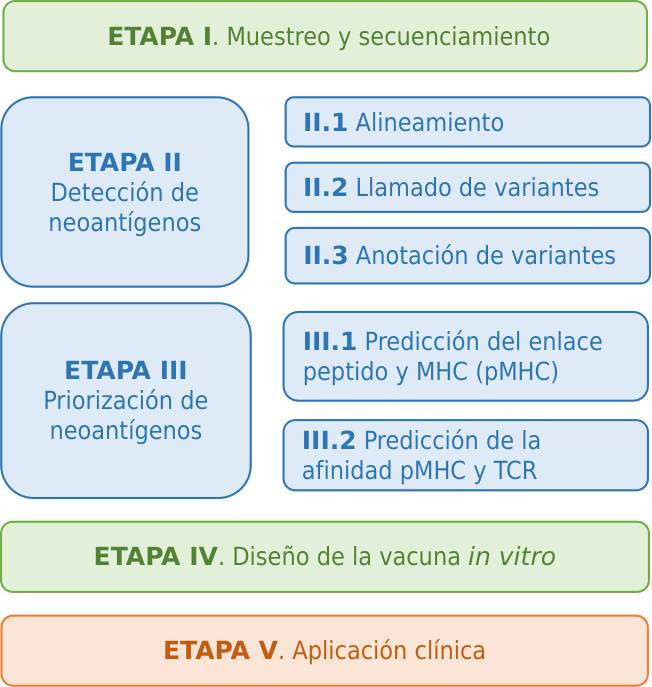
\includegraphics[width=0.4\textwidth]{../img/vaccines/pipeline2}	
	\caption{Marco de desarrollo para la elaboración de vacunas personalizadas contra el cáncer basadas en neoantígenos. Se detalla cada fase enfatizando el desarrollo \textit{in-silico}. Fuente: Elaboración propia.}
	\label{fig:vaccines}
\end{figure}
	
	
La detección \textit{in-silico} de neoantígenos se basa en la ETAPA II y III (ver Figura \ref{fig:vaccines} del material complementario). En este contexto, debido a la complejidad del proceso y la cantidad de métodos existentes, se han desarrollado software y \textit{pipelines} para facilitar el uso de estas herramientas. En la Tabla \ref{tab:review_pipelines} del material complementario, presentamos los \textit{pipelines} publicados a partir del 2018. Estos \textit{pipelines} utilizan diferentes tipos de información como entrada, así PGV Pipeline \cite{rubinsteyn2018computational} y PEPPRMINT \cite{zhou2023prioritizing} utilizan DNA-seq; sin embargo, otras herramientas como PGNneo \cite{tan2023pgnneo}, NAP-CNB \cite{wert2021predicting}, NaoANT-HILL \cite{coelho2020neoant}, ProGeo-neo \cite{li2020progeo}, ScanNeo \cite{wang2019scanneo} y Neopepse \cite{kim2018neopepsee} utilizan RNA-seq porque estas secuencias encapsulan mejor la información de mutaciones y \textit{non-coding regions} de ADN \cite{tan2023pgnneo}. 

Con el objetivo de reducir la complejidad de los \textit{pipelines}, otras propuestas han optado por utilizar Variant Calling Format (VCF), como entrada. Estos archivos, contienen información de las mutaciones y son obtenidas a partir de métodos de alineamiento y llamado de mutaciones (ETAPA II.1 y ETAPA II.3 de la Figura \ref{fig:vaccines} del material complementario). De esta forma, herramientas como Valid-Neo \cite{terai2022valid}, HLA3D \cite{li2022hla3d}, Neoepiscope \cite{wood2020neoepiscope} , pVACtools \cite{hundal2020pvactools} y NeoPredPipe \cite{schenck2019neopredpipe}, reducen la cantidad de herramientas utilizadas en la deteccion de neoantígenos; sin embargo, los resultados obtenidos, pueden ser inferiores comparado con herramientas que usan DNA-seq y RNA-seq. 

Adicionalmente, para una correcta detección de neoantígenos, es necesario contar con la secuenciación de proteínas Major Histocompatibility Complex (MHC) o Human Leukocyte Antigens (HLA). Es necesario contar con estas proteínas porque, son utilizadas para predecir la unión entre posibles neoantígenos al MHC (pMHC: ETAPA III.1 de la Figura \ref{fig:vaccines} del material complementario). Estas proteínas son codificadas por genes altamente polimórficos, esto proporciona una variación sustancial en la unión de péptidos (neoantígenos), influyendo de esta manera en el conjunto de péptidos presentados a las células T. \cite{abualrous2021major}. En este contexto,  los \textit{pipelines} Valid-NEO \cite{terai2022valid}  y NeoPredPipe \cite{schenck2019neopredpipe} y Neopepsee \cite{kim2018neopepsee} solicitan como entrada estas proteínas (HLA); mientras que las otras predicen esta información a partir de DNA-seq. Desde un punto de vista de usabilidad, obtener los tipos de HLA, implica un esfuerzo innecesario para el usuario.

%De esta la propuesta presenta una contribución en la disciplina de Bioinformática al plantear el uso de RNA-seq, DNA-seq en conjuno de datos Mass Spectrometry y además de que permiten predecir los tipos de proteínas HLA. Además, se va a incluir el uso de información de variaciones estructurales, fusión de genes y eventos de \textit{alternative splicing}. Estos fenómenos estan relacionados con varios tipos de cáncer \cite{wood2020neoepiscope} y aún no son utilizados por los pipelines estudiados en el estado del arte.  Finalmente, la propuesta presenta una contribución a la sub-area de Computación y Ciencias de la Información al incluir el desarrollo de un modelo \textit{Transformers} para la predicción del enlace pMHC y pMHC-TCR.  Este modelo aplicará fine-tuning de modelos BERT pre-entrenados en grandes bases de datos de proteínas. Según trabajos previos, los modelos Transformers obtienen mejores resultados que otras herramientas del estado del arte.
La presente propuesta ofrece una valiosa contribución a la disciplina de Bioinformática al proponer la integración de datos genómicos RNA-seq y DNA-seq, en combinación con datos de Mass Spectrometry.Además, también se va a incorporar información sobre variaciones estructurales, fusiones de genes y eventos de \textit{alternative splicing}, fenómenos que han sido vinculados a diversos tipos de cáncer \cite{wood2020neoepiscope} y que aún no son considerados por los pipelines examinados en el estado del arte. Adicionalmente, la propuesta presenta una contribución significativa en la sub-area de la Computación y Ciencias de la Información al introducir el desarrollo de un modelo basado en \textit{Transformers} para la predicción del enlace pMHC y pMHC-TCR. Este modelo empleará técnicas de fine-tuning utilizando modelos BERT pre-entrenados en extensas bases de datos de proteínas. Según investigaciones previas, los modelos Transformers han demostrado obtener resultados superiores en comparación con otras herramientas del estado del arte como NetMHCpan4.1 \cite{reynisson2020netmhcpan} y MHCflurry \cite{o2020mhcflurry}."


%En resumen, el desarrollo de \textit{pipelines} para la detección de neoantígenos es un campo de investigación significativo y de gran envergadura. Además, se está viendo favorecido por el crecimiento exponencial de la información genómica y los avances recientes en inteligencia artificial. 



% falta mencioan porque usan MS


	
\begin{table}[h]
	\caption{Lista de \textit{pipelines} desarrollados desde el 2018 hasta la actualidad para la detección de neoantígenos.GN: Expresión de genes, VA: anotación de variantes.}
	\label{tab:review_pipelines}
 \centering
	\setlength{\tabcolsep}{0.5em} % for the horizontal padding
	{\renewcommand{\arraystretch}{1.8}% for the vertical padding
    {\footnotesize
    \begin{tabular}{lllp{2cm}p{8.5cm}p{2cm}}
	\textbf{Nombre} & \textbf{Año}  & \textbf{Ref.}                                 & \textbf{Entrada}                                         & \textbf{Salida}    & \textbf{Herramientas}                                 \\ \hline
	
	PEPPRMINT         & 2023 &\cite{zhou2023prioritizing}         & DNA-seq                                                  & BWA, Mutect, Strelka, ANNOVAR, OptiType, PEPPRMINT, netMHCpan4.1 & Neoantígenos                                        \\

	PGNneo & 2023	& \cite{tan2023pgnneo}	& VCF, RNA-seq y MS data & Trimmomatic, BWA, SAMtools, GATK, Picard, OptiType, Annovar, Bedtools, MaxQuant, NetMHCpan4.1, Blastp	& Neoantígenos \\
	
	Valid-NEO       & 2022 &\cite{terai2022valid}             & VCF y HLA          & Neoantígenos  \\
	
	HLA3D & 2022	& \cite{li2022hla3d}	& VCF, HLA, SMG y HBV	& MHCcluster, SAVES, PROCHECK, CoDockPP, Verify 3D, ERRAT, ClusterW2, 3Dmol, PSRPRED4.0, MHCf lurry, CoDockPP & Neoantígenos \\
	
	
	
	NAP-CNB         & 2021 &\cite{wert2021predicting}         & RNA-seq                                                  & Star, Picard, GATK, SplitNCigarsReads, MuTect2, Cufinks, Epi-Seq, pVAC,seq, Neoantimon, MuPeXI, BLOSUM62 &  Neoantígenos                                       \\
	
	NeoANT-HILL     & 2020 &\cite{coelho2020neoant}           & RNA-seq y VCF                   & GATK, Mutect2, Optitype, NetMHC, NetMHCpan, NetMHCCcons, NetMHCstapan, PickPoket, SMM, SMMPMBEC, MHCflurry, NetMHCIIpan, NN-align, SMM-align, Sturniolo, Kallisto     & Neoantígenos,GE  \\
	
	Neoepiscope     & 2020 &\cite{wood2020neoepiscope}        & VCF y BAM            & BWA, Bowtie2, Pindel, MuSE, RADIA, SomaticSniper, VarScan2, GATK, HapCUT2       & Neoantígenos                          \\
	
	ProGeo-neo      & 2020 &\cite{li2020progeo}               & RNA-seq y VCF           & SRA Toolkit, BWA, GATK, Bcftools, ANNOVAR, Kallisto, OptiType, NetMHCpan4.0, Picard             & Neoantígenos                                       \\
	
	pVACtools       & 2020 &\cite{hundal2020pvactools}        & VCF                                         & CWL36, Cromwell37, ADNc38, BWA-MEM25, HaplotypeCaller28, MHCflurry14, MHCnuggets15, NetChop17, INTEGRATE-Neo19 & Neoantígenos                                       \\
	
	NeoPredPipe     & 2019 &\cite{schenck2019neopredpipe}     & VCF y HLA                & ANNOVAR, POLYSOLVER, netMHCpan, PeptideMatch            & Neoantígenos,VA              \\
	
	ScanNeo         & 2019 &\cite{wang2019scanneo}            & RNA-seq                                                  & HISAT2, BEDTools, BWA-MEM, pVAC-Seq, NetMHC, NetMHCpan & Neoantígenos                                       \\
	
		
	Neopepsee       & 2018 &\cite{kim2018neopepsee}           & RNA-seq, VCF, HLA  & NetCTLpan, Swiss-Prot & Neoantígenos,GE    \\ 
	
	PGV Pipeline    & 2018 &\cite{rubinsteyn2018computational}& DNA-seq                                                  & BWA-MEN, BQSR, MuTect, Strelka, STAR, seq2hla, Vaxrank, Isovar, MHCtools, Varcode, pyEnsembl & Neoantígenos                                       \\
	

\end{tabular}
}	
}
\end{table}



%\end{comment}

%\begin{comment}
\section{Resultados o avances previos (4k)}


%La propuesta del proyecto es la continuación de una serie de proyectos y publicaciones. Primero se inicio con el PROYECTO 01: ``Principales estrategias y métodos basados en deep learning para la detección de neoantígenos en el marco del desarrollo de vacunas personalizadas en la inmunoterapia del cáncer'' financiado por la Universidad La Salle y la Universidad Católica San Pablo. Este proyecto generó como resultado dos publicaciones: ``Deep Learning and Transformers in MHC-Peptide Binding and Presentation Towards Personalized Vaccines in Cancer Immunology: A Brief Review'' \cite{machaca2023deep} y ``Neoantigen Detection Using Transformers and Transfer Learning in the Cancer Immunology Context'' \cite{arceda2023neoantigen}. 
La propuesta del proyecto representa la continuación de una serie de iniciativas y publicaciones. Se inició con el PROYECTO 01: "Principales estrategias y métodos basados en deep learning para la detección de neoantígenos en el marco del desarrollo de vacunas personalizadas en la inmunoterapia del cáncer", financiado por las Universidades La Salle y Católica San Pablo. Este proyecto resultó en dos publicaciones: "Deep Learning and Transformers in MHC-Peptide Binding and Presentation Towards Personalized Vaccines in Cancer Immunology: A Brief Review" \cite{machaca2023deep} y "Neoantigen Detection Using Transformers and Transfer Learning in the Cancer Immunology Context" \cite{arceda2023neoantigen}.

%Tambien, recientemente hemos culminado la ejecución del PROYECTO 02: ``Desarrollo de una Aplicación Web para la Detección de Neoantígenos en el Marco de Desarrollo de Vacunas Personalizadas para Tratar el Cáncer'', en este proyecto estamos desarrollando una aplicación para la detección de neoantígenos, enfocados en la predicción del enlace pMHC utilizando modelos Transformers y Transfer Learning. Asu vez, hemos sometido a revisión el paper ``Fine-tuning Transformers for Peptide-MHC Class I Binding Prediction''. Adicionalmente, esta propuesta de PROCIENCIA es el trabajo futuro de la tesis de doctorado en Ciencia de la Computación del investigador principal Vicente Machaca Arceda. La tesis titula: ``Detección \textit{in Silico} de Neoantígenos Utilizando Transformers y Transfer Learning en el Marco de Desarrollo de Vacunas Personalizadas para Tratar el Cáncer''. En la tesis se desarrolló los mismos objetivos del PROYECTO 02. Además, se logró la aceptación del artículo ``Transformers Meets Neoantigen Detection: A Systematic Literature Review'' al Journal of Integrative Bioinformatics (Q2).

Recientemente, hemos completado la ejecución del PROYECTO 02: "Desarrollo de una Aplicación Web para la Detección de Neoantígenos en el Marco de Desarrollo de Vacunas Personalizadas para Tratar el Cáncer". En este proyecto, hemos creado una aplicación centrada en la detección de neoantígenos, con un enfoque en la predicción del enlace pMHC mediante el uso de modelos Transformers y Transfer Learning. Además, hemos enviado para revisión el artículo "Fine-tuning Transformers for Peptide-MHC Class I Binding Prediction". Además, esta propuesta de PROCIENCIA también representa el trabajo futuro de la tesis de doctorado en Ciencia de la Computación del investigador principal, Vicente Machaca Arceda, titulada: "Detección \textit{in Silico} de Neoantígenos Utilizando Transformers y Transfer Learning en el Marco de Desarrollo de Vacunas Personalizadas para Tratar el Cáncer". La tesis aborda los mismos objetivos que el PROYECTO 02 y ha logrado la aceptación del artículo "Transformers Meets Neoantigen Detection: A Systematic Literature Review" en el Journal of Integrative Bioinformatics (Q2).

%Finalmente, esta en ejecución el PROYECTO 03 ``NeoArgos-tools: Un Pipeline de Detección In-silico de Neoantígenos de Cáncer para el Desarrollo de Vacunas Personalizadas''. Este proyecto finaliza en Junio de este año y tambien es financiado por la Universidad La Salle y a UCSP. Este representa el desarrollo de la primera versión de NeoArgos-tools (esta postulación a PROCIENCIA representa la versión 2). En esta primera versión, tomamos como entrada archivos Variant Calling File (VCF) y hemos mejorado el modulo de predicción del enlace pMHC en base a investigaciones previas de proyectos anteriores. 
Actualmente, estamos llevando a cabo el PROYECTO 03 "NeoArgos-tools: Un Pipeline de Detección In-silico de Neoantígenos de Cáncer para el Desarrollo de Vacunas Personalizadas", con fecha de finalización en junio de este año y financiamiento de las Universidades La Salle y UCSP. Este proyecto implica el desarrollo de la versión inicial de NeoArgos-tools (la postulación a PROCIENCIA corresponde a la versión 2). En la primera versión, utilizamos archivos Variant Calling File (VCF) como entrada y mejoramos el módulo de predicción del enlace pMHC según investigaciones previas de proyectos anteriores.

%Es importante menconar que en esta versión 2 de NeoArgos-tools, las mejoras planteadas son: utilizar datos genómicos como entrada al pipeline (RNS-seq y DNA-seq), además vamos a utilizar Mass Spectrometry (MS) para afinar la detección de neoantígenos. Luego, tambien vamos a incluir información de variantes estructurales y fusión de genes. Finalmente, vamos a desarrollar una interfaz gráfica.
Es relevante destacar que en la versión 2 de NeoArgos-tools, las mejoras propuestas incluyen el uso de datos genómicos como entrada al pipeline (RNS-seq y DNA-seq), la incorporación de Mass Spectrometry (MS) para refinar la detección de neoantígenos, la inclusión de información sobre variantes estructurales y fusión de genes, y el desarrollo de una interfaz gráfica.





\section{Justificación (4k)}

%El cáncer es el mayor problema de salud mundial; sin embargo, los métodos tradicionales basados en cirugías, radioterapias y quimioterapias tienen baja efectividad \cite{peng2019neoantigen}. En este contexto, los neoantígenos son factores clave en el desarrollo de vacunas contra el Cáncer  \cite{borden2022cancer,chen2021challenges,gopanenko2020main}. Si se logra desarrollar un método con un buen desempeño, la inmunoterapia del cáncer basada en el desarrollo de vacunas personalizadas, podría utilizarse como alternativa a otros métodos como radioterapias y quimioterapias. 

%El proyecto tiene dos contribuciones: CONTRIBUCIÓN 01: En el área de ciencia de la computación se va a desarrollar un modelo basado en \textit{Transformers} y Transfer Learning para la predicción del enlace pMHC, actualmente se tienen resultados previos que superan a otros del estado del arte. CONTRIBUCIÓN 02: En el área de la Bioinformática: el desarrollo del \textit{pipeline}, representa un reto resolviendo problemas de integración, alto costo computacional, heterogeneidad y modularidad. Además,  el \textit{pipeline} utilizará datos de \textit{Mass Spectrometry} (MS) y fusión de genes para obtener mejores resultados que otros métodos del estado del arte.

%Finalmente, con la culminación de este este proyecto, vamos a proceder con la segunda parte que involucra un trabajo interdisciplinario para el desarrollo \textit{in vitro} de las vacunas de neoantígenos. En una tercera etapa, se plantearán pruebas clínicas.
El cáncer constituye el principal desafío de salud a nivel global; no obstante, las técnicas convencionales basadas en cirugías, radioterapias y quimioterapias presentan una eficacia limitada \cite{peng2019neoantigen}. En este escenario, los neoantígenos emergen como elementos cruciales en la concepción de vacunas contra el cáncer \cite{borden2022cancer,chen2021challenges,gopanenko2020main}. Si se logra desarrollar un enfoque altamente efectivo, la inmunoterapia del cáncer, fundamentada en la creación de vacunas personalizadas, podría posicionarse como una alternativa a procedimientos más tradicionales, como radioterapias y quimioterapias.

En el proyecto se propone realizar dos contribuciones significativas: CONTRIBUCIÓN 01: En el ámbito de la ciencia de la computación, se llevará a cabo el desarrollo de un modelo basado en \textit{Transformers} y Transfer Learning para la predicción del enlace pMHC, con resultados previos que demuestran superar a otras propuestas en el estado del arte. CONTRIBUCIÓN 02: En el ámbito de la Bioinformática, la implementación del \textit{pipeline} plantea un desafío al abordar problemas de integración, alto costo computacional, heterogeneidad y modularidad. Además, este \textit{pipeline} incorporará datos de \textit{Mass Spectrometry} (MS), variaciones estructurales y fusión de genes con el objetivo de obtener resultados más sobresalientes que otros métodos presentes en el estado del arte.

Con la conclusión de este proyecto, se abrirá paso a la segunda fase, que implica una colaboración interdisciplinaria para llevar a cabo el desarrollo \textit{in vitro} de las vacunas de neoantígenos. En una tercera etapa, se contemplarán pruebas clínicas, marcando así un avance integral en la búsqueda de soluciones efectivas en la lucha contra el cáncer.







\section{Porqué es una investigación básica (3k)}

A partir del conocimiento en el estado del arte en el área de inmunoterapia para tratamiento de cáncer se tiene que:

\begin{itemize}
	

\item Existen varios tratamientos: vacunas personalizadas, terapias con células T adoptivas, inhibidores de puntos de control inmunológico, de los cuales, es más promisorio el uso de vacunas basadas en neo antígenos.
\item A pesar de los esfuerzos realizados, los neoantígenos alcanzan un nivel de efectividad de activación del sistema inmune menor a apenas 5%.
\item Se tiene algunas explicaciones para esta poca efectividad como falta de más fuentes de información: DNA-Seq, RNA-Seq, datos de Espectrometría de Masas, siendo que la cantidad de esta información es creciente y se utiliza en otros campos.
\item Las herramientas encontradas para la predicción de los enlaces péptidos-MHC (pMHC) son poco efectivas.
\item Aún no se está aprovechando la información de splicing alternativo ni variaciones estructurales en el ADN, y esta información está bastante ligada a varios tipos de cáncer.
\end{itemize}

Además, se tiene en el estado del arte que ya se ha cuenta con una metodología para el proceso de desarrollo de vacunas personalizadas, denominada pipeline que se seguirá en la investigación proponiendo algunas novedades de contribución en el proceso tales como:

\begin{itemize}


\item Desarrollo de un modelo basado en el modelo Transformers de Inteligencia Artificial, Deep Learning que actuará como predictor del enlace pMHC, que en resultados previos ha mostrado mejores resultados a propuestas en el estado del arte.
\item Incorporación de datos de Espectrometría de Masas (MS), variaciones estructurales y fusión de genes apuntando a lograr resultados más interesantes que los métodos del estado del arte.
\end{itemize}

Es así que con esta propuesta se cumplen los requisitos de una investigación básica:

\begin{itemize}
\item Obtención de nuevos conocimientos tanto teóricos como experimentales en la implementación de los pipelines para obtención de vacunas personalizadas al incluir nuevas técnicas y verificar sus comportamientos e impactos en los resultados obtenidos. 
\item Aunque existe una área de aplicación definida (pipeline de vacunas basadas en neo antígenos), se está probando técnicas que se avizora podrían obtener resultados interesantes, pero aún no se hicieron pruebas ni análisis, con los cuales se espera obtener nuevos conocimientos para solucionar de mejor forma una etapa del problema de obtención de vacunas de neoantígenos. Así, esta propuesta calificaría como Investigación Básica Orientada.

\item Esta propuesta se alinea con la sub área de ciencias naturales en la disciplina de Ciencias de la Computación en Bioinformática, dado que propone verificar el comportamiento de técnicas del área de Ciencia de la Computación (Inteligencia Artificial, Deep Learning, Modelos Transformer) en problemas del área Bioinformática y Biología Computacional.
\end{itemize}
	
\section{Pregunta de investigación}	

¿El desarrollo de una herramienta in silico para la detección de neoaatígenos a partir de datos genómicos es capaz de detectar correctamente neoantígenos de cáncer?
	
\section{Objetivos de la investigación}
	
	\subsection{Objetivo general}
	
	Desarrollar una herramienta  para la detección \textit{in silico} de neoantígenos de cáncer a partir de datos genómicos.
	
	\subsection{Objetivos específicos}
	\begin{enumerate}
		\item \textbf{OBJ 1:} Evaluar alternativas para la integración de datos Mass Spectrometry (MS) con datos genómicos como RNA-seq y DNA-seq. 
		
		\item \textbf{OBJ 2:} Evaluar las herramientas STAR \cite{dobin2013star}, BWA \cite{li2009fast}, Bowtie2 \cite{langmead2019scaling} y Samtools \cite{danecek2021twelve} para determinar su aplicación en el alineamiento de secuencias.
		
		\item \textbf{OBJ 3:}
		Evaluar las herramientas GATK \cite{auwera2017somatic} y BFCtools \cite{danecek2021twelve} y determinar el uso apropiado de estas en el llamado de variantes. 
		
	
		
		\item \textbf{OBJ 4:} Analizar el uso de información de variaciones estructurales del ADN y mutaciones de fusión de genes. Se evaluará el desempeño de \textit{Arriba} \cite{uhrig2021accurate} y FusionQ \cite{liu2013fusionq}.


			\item \textbf{OBJ 5:} Evaluar la herramienta Isovar \cite{isovar2023} y Annovar \cite{wang2010annovar} para la anotación de variantes y la herramienta OptiType \cite{szolek2014optitype} para la predicción de tipos de HLA.
        %\item Evaluar métodos de detección de eventos de \textit{alternative splicing} y analizar la aplicación de estos al integrarse a la herramienta para la detección de neoantígenos.
		 
		\item \textbf{OBJ 6:} Implementar un modelo basado en \textit{transformers} para la predicción del enlace pMHC, esto como alternativa a NetMHCpan4.1 \cite{reynisson2020netmhcpan} o MHCflurry \cite{o2020mhcflurry}. Ya se cuenta con resultados previos de una propuesta que es superior a otras del estado del arte \cite{arceda2023neoantigen}.

        \item \textbf{OBJ 7:} Evaluar el modelo basado en \textit{transformers} para la predicción del enlace pMHC en otra tarea similar: la predicción  del enlace pMHC al TCR (pMHC-TCR). 
        
        \item \textbf{OBJ 8:} Implementar una interfaz gráfica que sirva como panel de administración para configurar y escoger las herramientas en cada fase del \textit{pipeline}.
		
        \item \textbf{OBJ 9:} Comparar el desempeño de la herramienta propuesta con otras herramientas del estado del arte.

		
	\end{enumerate}


%\end{comment}



\begin{comment}
\section{Introducción} 


El desarrollo de vacunas personalizadas contra el cáncer es un proceso largo y depende de la correcta detección de neoantígenos (ver Figura \ref{fig:vaccines} del material complementario). Estos neoantígenos son péptidos que solo están presentes en las células cancerosas. De esta forma, el objetivo de un tratamiento basado en vacunas personalizadas, es entrenar a los linfocitos del paciente (células T) para reconocer los neoantígenos y activar el sistema inmunológico \cite{de2020neoantigen, peng2019neoantigen}. El proceso consiste en: 




\begin{enumerate}
	\item ETAPA I: Obtener muestras de tejido canceroso y saludable, Luego se secuencia ambos tejidos para obtener el ADN y/o ARN. Algunas propuestas incluyen información inmunopeptidoma de \textit{Mass Spectrometry} (MS).
	\item ETAPA II: Aquí realiza alineamiento de secuencias, se desarrolla un \textit{llamado de variantes} para detectar las variantes y/o mutaciones; y se anotan dichas variantes (detección de posibles neoantígenos). Esta etapa cuenta con varias herramientas con buen desempeño.
	\item ETAPA III: En esta etapa \textit{in-silico} se priorizan neoantígenos. Esta etapa es crucial y ha tenido bastante investigación los últimos años debido a su complejidad y la baja efectividad de propuestas actuales. Aquí, se toman los neoantígenos candidatos (péptidos) de la etapa anterior y se predice su afinidad con el \textit{Major Histocompatibility Complex} (MHC), este problema se conoce como \textit{pMHC binding}. Luego, se  evalúa la afinidad del pMHC para enlazarse al T-cell Receptor (TCR). Al finalizar esta etapa, se obtienen los neoantígenos.
	\item ETAPA IV: En esta etapa \textit{in-vitro}, se induce en laboratorio  a las células T del paciente a reconocer los neoantígenos. Aquí, se desarrollan las vacunas. Generalmente, esta etapa es desarrollada por biotecnólogos y biólogos.
	\item ETAPA V: Finalmente, el médico oncólogo realiza la evaluación clínica de la vacuna.
\end{enumerate}



\begin{figure}[H]	
	\centering
	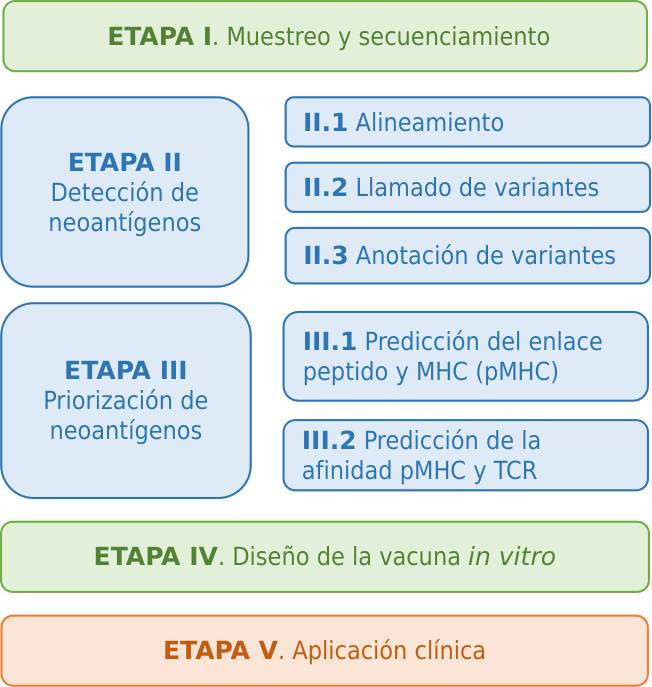
\includegraphics[width=0.5\textwidth]{../img/vaccines/pipeline2}	
	\caption{Marco de desarrollo para la elaboración de vacunas personalizadas contra el cáncer basadas en neoantígenos. Se detalla cada fase enfatizando el desarrollo \textit{in-silico}. Fuente: Elaboración propia.}
	\label{fig:vaccines}
\end{figure}


Las principales \textit{pipelines} desarrollados hasta la actualidad para la detección de neoantígenos son detallados en la Tabla \ref{tab:review_pipelines}.

\begin{table}[h]
	\caption{Lista de \textit{pipelines} desarrollados desde el 2018 hasta la actualidad para la detección de neoantígenos.GN: Expresión de genes, VA: anotación de variantes.}
	\label{tab:review_pipelines}
	\centering
	\setlength{\tabcolsep}{0.5em} % for the horizontal padding
	{\renewcommand{\arraystretch}{1.8}% for the vertical padding
		{\footnotesize
			\begin{tabular}{lllp{2cm}p{8.5cm}p{2cm}}
				\textbf{Nombre} & \textbf{Año}  & \textbf{Ref.}                                 & \textbf{Entrada}                                         & \textbf{Salida}    & \textbf{Herramientas}                                 \\ \hline
				
				PEPPRMINT         & 2023 &\cite{zhou2023prioritizing}         & DNA-seq                                                  & BWA, Mutect, Strelka, ANNOVAR, OptiType, PEPPRMINT, netMHCpan4.1 & Neoantígenos                                        \\
				
				PGNneo & 2023	& \cite{tan2023pgnneo}	& VCF, RNA-seq y MS data & Trimmomatic, BWA, SAMtools, GATK, Picard, OptiType, Annovar, Bedtools, MaxQuant, NetMHCpan4.1, Blastp	& Neoantígenos \\
				
				Valid-NEO       & 2022 &\cite{terai2022valid}             & VCF y HLA          & Neoantígenos  \\
				
				HLA3D & 2022	& \cite{li2022hla3d}	& VCF, HLA, SMG y HBV	& MHCcluster, SAVES, PROCHECK, CoDockPP, Verify 3D, ERRAT, ClusterW2, 3Dmol, PSRPRED4.0, MHCf lurry, CoDockPP & Neoantígenos \\
				
				
				
				NAP-CNB         & 2021 &\cite{wert2021predicting}         & RNA-seq                                                  & Star, Picard, GATK, SplitNCigarsReads, MuTect2, Cufinks, Epi-Seq, pVAC,seq, Neoantimon, MuPeXI, BLOSUM62 &  Neoantígenos                                       \\
				
				NeoANT-HILL     & 2020 &\cite{coelho2020neoant}           & RNA-seq y VCF                   & GATK, Mutect2, Optitype, NetMHC, NetMHCpan, NetMHCCcons, NetMHCstapan, PickPoket, SMM, SMMPMBEC, MHCflurry, NetMHCIIpan, NN-align, SMM-align, Sturniolo, Kallisto     & Neoantígenos,GE  \\
				
				Neoepiscope     & 2020 &\cite{wood2020neoepiscope}        & VCF y BAM            & BWA, Bowtie2, Pindel, MuSE, RADIA, SomaticSniper, VarScan2, GATK, HapCUT2       & Neoantígenos                          \\
				
				ProGeo-neo      & 2020 &\cite{li2020progeo}               & RNA-seq y VCF           & SRA Toolkit, BWA, GATK, Bcftools, ANNOVAR, Kallisto, OptiType, NetMHCpan4.0, Picard             & Neoantígenos                                       \\
				
				pVACtools       & 2020 &\cite{hundal2020pvactools}        & VCF                                         & CWL36, Cromwell37, ADNc38, BWA-MEM25, HaplotypeCaller28, MHCflurry14, MHCnuggets15, NetChop17, INTEGRATE-Neo19 & Neoantígenos                                       \\
				
				NeoPredPipe     & 2019 &\cite{schenck2019neopredpipe}     & VCF y HLA                & ANNOVAR, POLYSOLVER, netMHCpan, PeptideMatch            & Neoantígenos,VA              \\
				
				ScanNeo         & 2019 &\cite{wang2019scanneo}            & RNA-seq                                                  & HISAT2, BEDTools, BWA-MEM, pVAC-Seq, NetMHC, NetMHCpan & Neoantígenos                                       \\
				
				
				Neopepsee       & 2018 &\cite{kim2018neopepsee}           & RNA-seq, VCF, HLA  & NetCTLpan, Swiss-Prot & Neoantígenos,GE    \\ 
				
				PGV Pipeline    & 2018 &\cite{rubinsteyn2018computational}& DNA-seq                                                  & BWA-MEN, BQSR, MuTect, Strelka, STAR, seq2hla, Vaxrank, Isovar, MHCtools, Varcode, pyEnsembl & Neoantígenos                                       \\
				
				
			\end{tabular}
		}	
	}
\end{table}
\end{comment}
%%%%%%%%%%%%%%%%%%%%%%%%%%%%%%%%

\section{Metodología} 


Hemos dividido la propuesta en dos módulos: NeoArgosMut y NeoArgosAntigen. NeoArgosMut, se enfoca en el llamado y anotación de variantes, obteniéndose como salida neoantígenos candidatos. Luego, NeoArgosAntigen, prioriza estos antígenos, al predecir su afinidad al MHC (pMHC) y luego la afinidad del pMHC al TCR (pMHC-TCR). En la Figura \ref{fig:pipeline} del material complementario, mostramos estos módulos. 



\begin{figure}[h]	
		\centering
		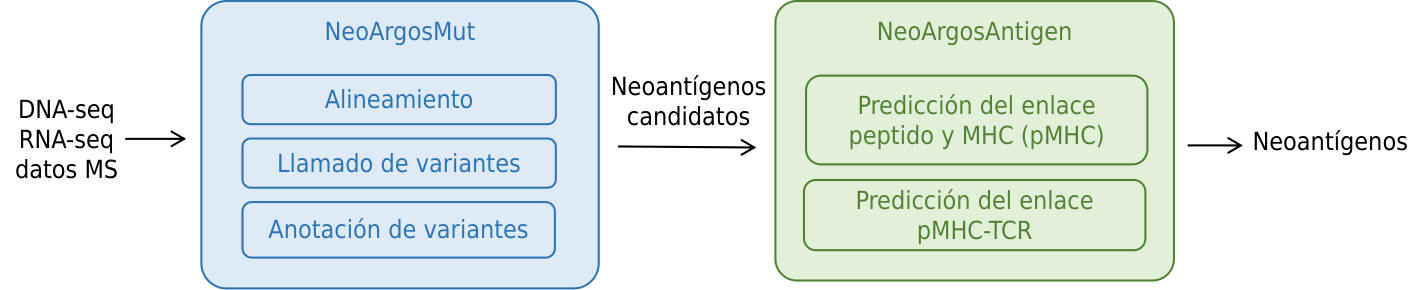
\includegraphics[width=\textwidth]{../img/pipeline/proposal_pipeline}	
	\caption{Representación de NeoArgosMut y NeoArgosAntigen para la detección de neoantígenos}
	\label{fig:pipeline}
\end{figure}


\subsection{NeoArgosMut}

Los objetivos específicos OBJ 1, OBJ  2, OBJ 3, OBJ 4 y OBJ 5 serán desarrollados con este modulo. Así, para el objetivo específico OBJ 1, NeoArgosMut, se encargará de recibir como entrada datos de DNA-seq, RNA-seq y Mass Spectrometry (MS). Se plantea utilizar la herramienta MaxQuant \cite{prianichnikov2020maxquant} para identificar las mutaciones a nivel de péptidos con ayuda de información de Mass Spectrometry (MS), esto  forma parte de la contribución del trabajo al incluir fuentes adicionales de información como MS.


Referente al objetivo específico OBJ 2, se plantea alinear las secuencias con uso de las herramientas BWA \cite{li2009fast}, Bowtie2 \cite{langmead2019scaling} y Samtools \cite{danecek2021twelve}. Adicionalmente, se planteará utilizar STAR, porque alinea mejor muestras tumorales \cite{rubinsteyn2018computational}. En esta etapa, se analizará y se determinará la mejor configuración y uso de cada herramienta. Como salida a esta etapa, se obtiene archivos de alineamiento BAM.



Para el objetivo específico OBJ 3 que corresponde al llamado de variantes se utilizará MuTect y Strelka. Se plantea usar la unión de la información de ambos métodos tal como lo hizo \cite{zhou2023prioritizing} y \cite{rubinsteyn2018computational}. Como salida, se obtienen archivos VCF. Adicionalmente a otros \textit{pipelines}, en esta etapa también abordaremos el objetivo especifico OBJ 4 y utilizaremos información sobre la fusión de genes que se obtendrán de las herramientas \textit{Arriba} \cite{uhrig2021accurate} y FusionQ \cite{liu2013fusionq}. Esta forma parte de la contribución de este trabajo, porque se sabe que la mayoría de \textit{pipelines} tienen un bajo desempeño debido ausencia de información en su procesos de variantes estructurales y fusión de genes \cite{wood2020neoepiscope}. 



Finalmente el objetivo específico OBJ 5, se enfoca en la anotación de variantes y predicción del tipo de HLA. En esta etapa se toman los archivos en formato VCF y se obtienen los péptidos generados a partir de estas variaciones o mutaciones. Estos péptidos representan los posibles neoantígenos. Para está tarea se va a utilizar Isovar \cite{isovar2023} y ANNOVAR \cite{wang2010annovar}, se evaluará su desempeño y se determinará cual de ellas usar bajo varios contextos. Luego, para obtener el tipo de HLA del paciente se va a utilizar la herramienta OptiType \cite{szolek2014optitype}. Otros \textit{pipelines} optan por solicitar al usuario la información del tipo de HLA; sin embargo, obtener el HLA a partir de las mismas secuencias de ADN, mejora considerablemente el desempeño general del pipeline y la accesibilidad del usuario. Al  finalizar esta etapa, se va a obtener los neoantígenos candidatos y los tipos de HLA.


\subsection{NeoArgosAntigen}

Los objetivos específicos OBJ 6, OBJ  7, OBJ 8, y OBJ 9 serán desarrollados con este modulo. NeoArgosAntigen, toma como entrada los neoantígenos candidatos y los tipos de HLA generados por NeoArgosMut. Esta prioriza estos neoantígenos. Esta priorización la realiza en base a la predicción del enlace de los neoantígenos al MHC, también conocido como predicción del enlace pMHC. Posteriormente se plantea predecir la afinidad del pMHC al TCR. El módulo se divide en dos partes: la predicción del enlace pMHC y la afinidad del pMHC al TCR. Ambas toman como entrada dos secuencias de proteínas, luego se necesita predecir su afinidad (regresión) o el enlace (clasificación). En resumen, las proteínas se pueden representar como $p = \{ A, ... , Q \}$ y $q = \{ A, N, ... ,Q, E, G \}$. Luego, tenemos que  predecir la probabilidad del enlace o afinidad entre $p$ y $q$. 


\begin{figure}[H]
	\centering
	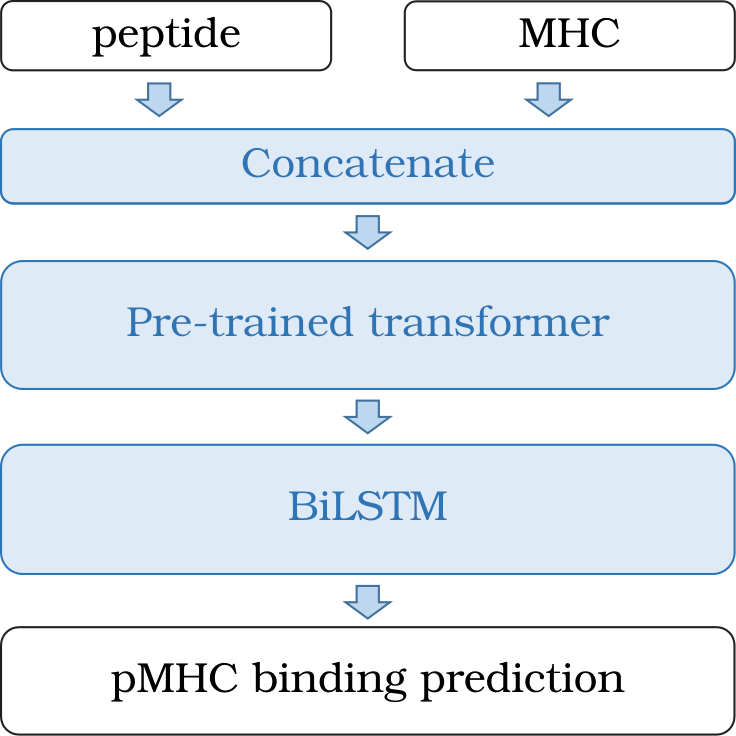
\includegraphics[width=0.30\textwidth]{../img/pipeline/proposal_pmhc}
	\caption{Modelo  \textit{transformer} seguido de BiLSTM para predecir el enlace pMHC.}
	\label{fig:proposal}
\end{figure}



Referente al objetivo específico OBJ 6, sobre el problema de predicción del enlace pMHC, se va a utilizar modelos BERT pre-entrenados y se realizará \textit{fine-tuning} agregando un bloque de capas BiLSTM, y otra basada en grafos. Luego se volverá a entrenar estos modelos con una base de datos compuesta por muestras de \cite{zhang2022hlab} y \cite{gfeller2023improved}. Se propone la arquitectura de la Figura \ref{fig:proposal} del material complementario. Como se puede ver, la entrada son dos secuencias de proteínas: el péptido y el MHC. Luego, el modelo basado en Transformers está compuesto por un modelo pre-entrenado y un bloque de capas BiLSTM, esta propuesta se basó en el trabajo de \cite{zhang2022hlab}. En esta etapa también. se va a evaluar el desempeño de varios modelos BERT pre-entrenados como: TAPE \cite{rao2019evaluating}, ProtBERT-BFD \cite{elnaggar2021prottrans} y ESM2 \cite{lin2023evolutionary} cada una con 92 millones, 420 millones, 650 millones parámetros respectivamente. Adicionalmente, TAPE fue entrenado con 30 millones de proteínas, ProtBERT-BFD con 2122 millones de proteínas y 60 millones de proteínas para ESM-2. En base a trabajos anteriores propios, sabemos que el uso de TAPE y el modelo más pequeño de ESM2 tienen buenos resultados \cite{arceda2023neoantigen}. Además, por investigaciones previas propias sabemos que podemos superar el desempeño de las mejores herramientas del estado del arte como NetMHCpan4.1 \cite{reynisson2020netmhcpan} y MHCflurry \cite{o2020mhcflurry}.



Para el objetivo específico OBJ 7 para la predicción del enlace pMHC y TCR (pMHC-TCR), se utilizará la misma metodología del objetivo 6, según recomendaciones de otros autores \cite{li2020progeo, myronov2023bertrand}. Sin embargo, se va reentrenar el modelo para adaptarse a este nuevo problema, se utilizarán muestras de \cite{li2020progeo} y la base de datos de VDJdb \cite{shugay2018vdjdb}. Al finalizar esta etapa, se obtendrán los neoantígenos priorizados.


Luego, para lograr el objetivo especifico OBJ 8 referente al desarrollo de una interfaz gráfica para la configuración y selección de herramientas se va a desarrollar una herramienta similar a Orange Machine Learning. Por ejemplo, en la Figura \ref{fig:gui} del material complementario se muestra el prototipo de la interfaz gráfica. En el panel izquierdo se muestran las posibles herramientas, de las cuales el usuario podrá escoger y configurar. En color azul, se resaltan las herramientas que representan una contribución en este trabajo. Luego, en el panel derecho, se muestra como el usuario puede realizar el flujo de actividades con las herramientas que ha seleccionado.

Finalmente, para lograr desarrollar el objetivo especifico OBJ 9, se va a comparar el resultado de la propuesta con otros pipelines del estado del arte. En la Tabla \ref{tab:review_pipelines} del material complementario se detallan estas herramientas. La comparación se realizará con las herramientas PEPPRMINT, HLA3d, ProGeoNeo y pVACtools. 



\begin{figure}[H]
	\centering
	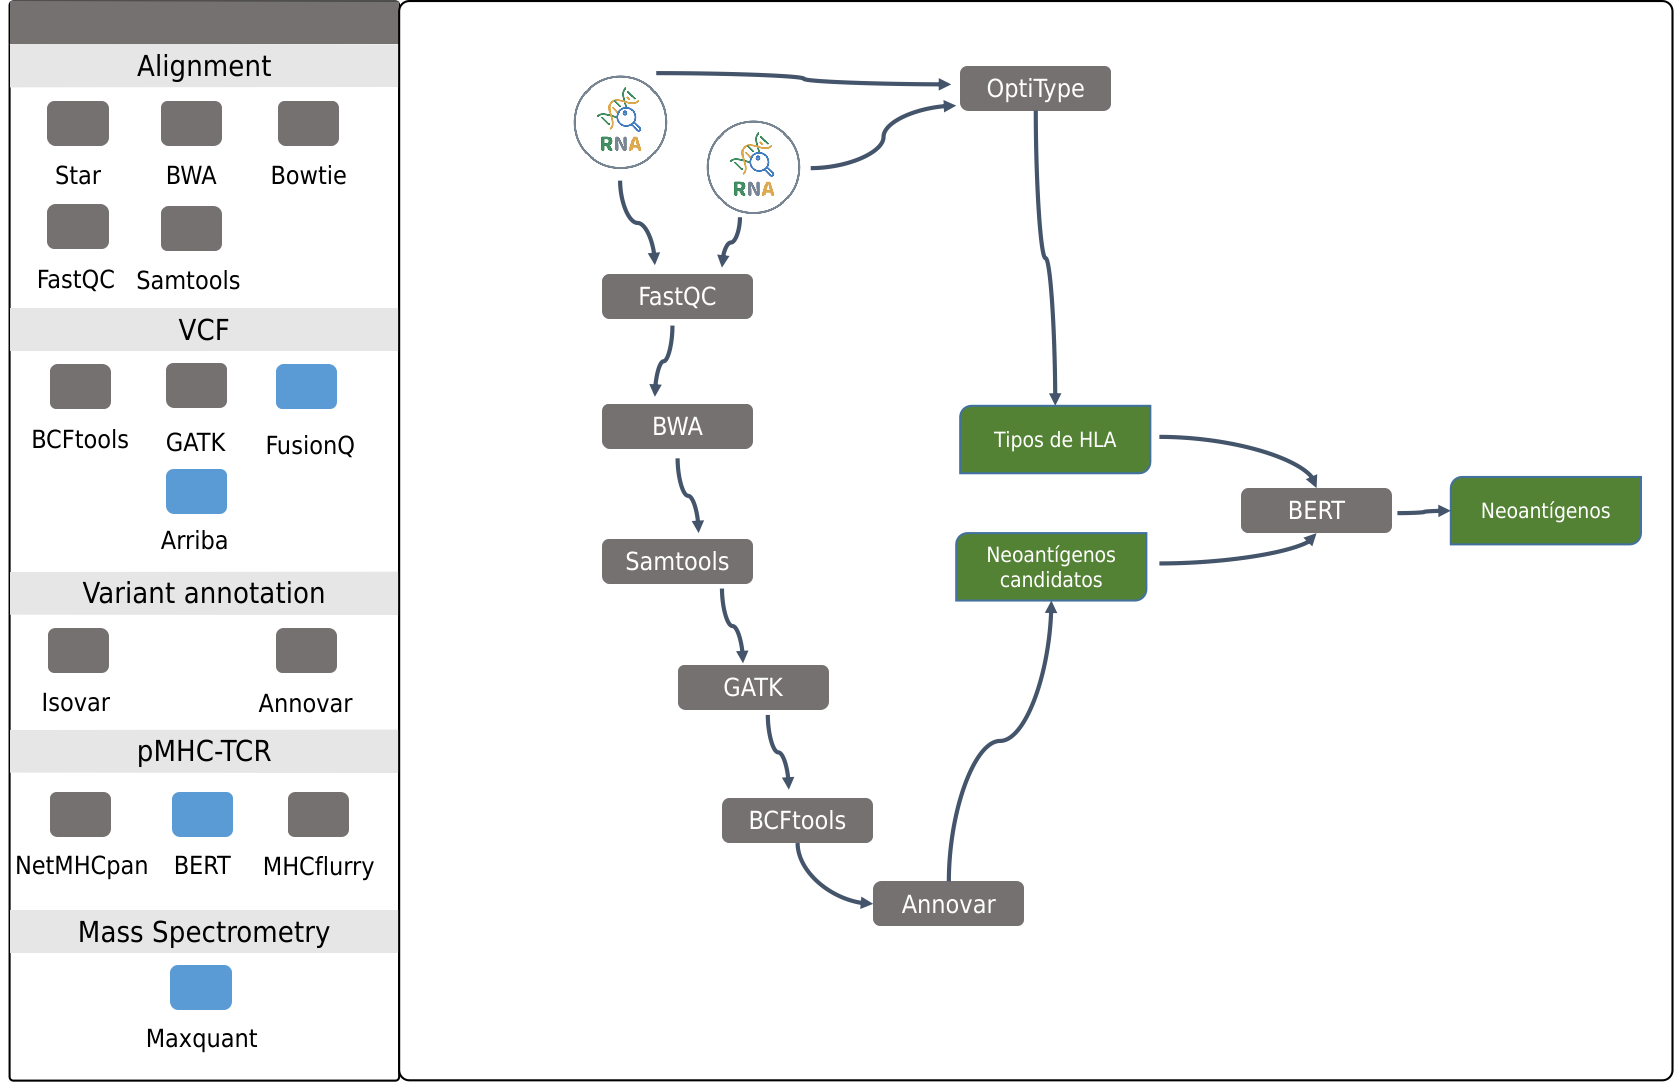
\includegraphics[width=\textwidth]{../img/proposal/gui2}
	\caption{Prototipo de la interfaz gráfica de la herramienta para la detección de neoantígenos. En el panel izquierdo se muestran las posibles herramientas, de las cuales el usuario podrá escoger y configurar. En color azul, se resaltan las herramientas que representan una contribución en este trabajo. Luego, en el panel derecho, se muestra como el usuario puede realizar el flujo de actividades con las herramientas que ha seleccionado.}
	\label{fig:gui}
\end{figure}




\section{Limitaciones (5K)}

En el estado del arte se observa que la efectividad de la detección de neoantígenos es aún muy baja, en ese sentido se está proponiendo aplicar estrategias que involucren técnicas y métodos novedosos apuntando a aumentar esta efectividad. Con todo, no es posible en este momento colocar una meta deseada (10\%, 20\%) a alcanzar por lo que queda algo difuso definir un umbral de éxito o fracaso del proyecto. La confianza que se tiene en alcanzar resultados satisfactorios es que se está planteando el uso de más informaciones y también técnicas de IA más potentes que han logrado resultados muy interesantes en el estado del arte de problemas relacionados. 

Adicionalmente, el alcance de este proyecto está determinado por el software desarrollado, este software (pipeline) NeoArgosTools, tendrá la funcionalidad de detectar neoantígenos a partir de datos genómicos. En nuestra planificación, el siguiente paso es continuar con el desarrollo de las vacunas in vitro y las pruebas clínicas, esta fase está fuera del alcance del proyecto y es un trabajo interdisciplinario y será desarrollado en un futuro cercano.

Adicionalmente en asuntos más operativos se consideran los siguientes riesgos y estrategias para mitigarlos:

Retraso con la adquisición de equipos (Workstation). En este caso, este proyecto depende mucho de contar con equipos de alto rendimiento y no tenerlos a tiempo, pondría en riesgo la completitud del proyecto. Sin embargo, actualmente la Universidad La Salle cuenta con créditos en las plataformas Paperspace y DigitalOceam, estas 




\section{Resultados esperados}

Un articulo en un Journal, un artícuo en una conferencia, una tesis lista para sustentar.



\section{Cronograma de Actividades}



	


% Please add the following required packages to your document preamble:
% \usepackage{multirow}


\begin{table}[H]
	\scriptsize
	\begin{tabular}{p{0.6cm}p{0.6cm}p{6cm}p{4cm}p{1cm}cccccc} \\ \hline
		
		
		
		
		
		\textbf{Hito}        & \textbf{Fases}        & \textbf{Objetivos específicos}                                                                                                                                                                                                                                                             & \textbf{Actividades}                                                                                 & \textbf{Encargado} & \multicolumn{1}{c}{I} & \multicolumn{1}{c}{II} & III                  & IV                   & \multicolumn{1}{c}{V} & \multicolumn{1}{c}{VI} \\  \hline
		
		\multirow{17}{*}{I}  & \multirow{3}{*}{I.1}  & \multirow{3}{6cm}{OBJ 1: Evaluar alternativas para la integración de datos Mass Spectrometry (MS) con datos genómicos como RNA-seq y DNA-seq.}                                                                                                                                            & Investigar y evaluar el uso de RNA-se y DNA.seq                                                      & Vicente            & \multicolumn{1}{c}{x} & \multicolumn{1}{c}{x}  & \multicolumn{1}{l}{} & \multicolumn{1}{l}{} &                       &                        \\
		
		&                       &                                                                                                                                                                                                                                                                                            & Evaluar herramientas para tratar datos de MS                                                         &                    &                       & \multicolumn{1}{c}{x}  & x                    & x                    & \multicolumn{1}{c}{x} &                        \\
		&                       &                                                                                                                                                                                                                                                                                            & Integración de datos  MS y RNA-seq                                                                   & Yvan               &                       &                        & x                    & x                    & \multicolumn{1}{c}{x} &                        \\ 
		& \multirow{5}{*}{I.2}  & \multirow{2}{6cm}{OBJ 2: Evaluar las herramientas STAR {[}36{]}, BWA {[}37{]}, Bowtie2 {[}38{]} y Samtools {[}39{]} para determinar su aplicación en el alineamiento de secuencias.}                                                                                                      & Evaluar y comparar cada herramienta de alineamiento                                                  & Tesista            & \multicolumn{1}{c}{x} & \multicolumn{1}{c}{x}  & x                    & x                    &                       &                        \\
		
		&                       &                                                                                                                                                                                                                                                                                            & Investigar sobre buenas prácticas y estandares                                                       &                    & \multicolumn{1}{c}{x} & \multicolumn{1}{c}{x}  & x                    & x                    &                       &                        \\
		&                       & \multirow{3}{6cm}{OBJ 3: Evaluar las herramientas GATK {[}40{]} y BFCtools {[}39{]} y determinar el uso apropiado de estas en el llamado de variantes.}                                                                                                                                   & Investigar sobre las buenas prácticas de GATK                                                        & Julio              &                       & \multicolumn{1}{c}{x}  & x                    & \multicolumn{1}{l}{} &                       &                        \\
		
		&                       &                                                                                                                                                                                                                                                                                            & Evaluar y comparar la herramienta GATK                                                               & Tesista            &                       & \multicolumn{1}{c}{x}  & x                    & x                    &                       &                        \\
		&                       &                                                                                                                                                                                                                                                                                            & Evaluar la herramienta BCFtools                                                                      & Tesista            &                       &                        & x                    & x                    &                       &                        \\
		& \multirow{4}{*}{I.3}  & \multirow{4}{6cm}{OBJ 4: Analizar el uso de información de variaciones estructurales del ADN y mutaciones de fusión de genes. Se evaluará el desempeño de Arriba [41] y FusionQ [42].}                                                                                            & Investigar sobre variaciones estructurales y fusión de genes                                         & Yvan               & \multicolumn{1}{c}{x} & \multicolumn{1}{c}{x}  & x                    & x                    & \multicolumn{1}{c}{x} &                        \\
		&                       &                                                                                                                                                                                                                                                                                            & Evaluar la herramienta Arriba                                                                        & Vicente            &                       &                        & x                    & \multicolumn{1}{l}{} &                       &                        \\
		&                       &                                                                                                                                                                                                                                                                                            & Evaluar la herramienta FusionQ                                                                       & Vicente            &                       &                        & x                    & \multicolumn{1}{l}{} &                       &                        \\
		&                       &                                                                                                                                                                                                                                                                                            & Investigar sobre otras herramientas para la detección de fusion de genes y variaciones estructurales & Yvan               &                       & \multicolumn{1}{c}{x}  & x                    & x                    & \multicolumn{1}{c}{x} &                        \\
		& \multirow{5}{*}{I.4}  & \multirow{5}{6cm}{OBJ 5: Evaluar la herramienta Isovar {[}43{]} y Annovar {[}44{]} para la anotación de variantes y la herramienta OptiType {[}45{]} para la predicción de tipos de HLA.}                                                                                                 & Evaluar la herramienta OptiType y semejantes                                                         & Yvan               &                       &                        & x                    & x                    &                       &                        \\
		&                       &                                                                                                                                                                                                                                                                                            & Evaluar la herramienta Isovar                                                                        &                    &                       &                        & x                    & \multicolumn{1}{l}{} &                       &                        \\
		&                       &                                                                                                                                                                                                                                                                                            & Evaluar la herramienta Annovar                                                                       &                    &                       &                        & x                    & \multicolumn{1}{l}{} &                       &                        \\
		&                       &                                                                                                                                                                                                                                                                                            & Investigar sobre otras herramientas y realizar comparaciones                                         & Yvan               &                       &                        & x                    & x                    &                       &                        \\
		&                       &                                                                                                                                                                                                                                                                                            & Integrar las herramientas en NeoArgosMut                                                             &                    &                       &                        & x                    & x                    & \multicolumn{1}{c}{x} &                        \\ \hline \hline
		\multirow{12}{*}{II} & \multirow{5}{*}{II.1} & \multirow{3}{6cm}{OBJ 6: Implementar un modelo basado en transformers para la predicción del enlace pMHC.} & Implementar el modelo basado en Transformers                                                         & Vicente            & \multicolumn{1}{c}{x} & \multicolumn{1}{c}{x}  & x                    & \multicolumn{1}{l}{} &                       &                        \\
		&                       &                                                                                                                                                                                                                                                                                            & Entrenamiento del modelo                                                                             & Vicente            &                       & \multicolumn{1}{c}{x}  & x                    & x                    &                       &                        \\
		&                       &                                                                                                                                                                                                                                                                                            & Evaluar el desempeño y comparar con otras herramientas                                               & Vicente            &                       & \multicolumn{1}{c}{x}  & x                    & x                    &                       &                        \\
		&                       & \multirow{2}{6cm}{OBJ 7: Evaluar el modelo basado en transformers para la predicción del enlace pMHC en otra tarea similar: la predicción del enlace pMHC al TCR.}                                                                                                             & Entrenar el modelo en bases de datos pMHC-TCR                                                        & Vicente            &                       &                        & x                    & x                    &                       &                        \\
		&                       &                                                                                                                                                                                                                                                                                            & Comparar el modelo con otras herramientas                                                            & Vicente            &                       &                        & \multicolumn{1}{l}{} & x                    &                       &                        \\
		& \multirow{3}{*}{II.2} & \multirow{3}{6cm}{OBJ 8: Implementar una interfaz gráfica que sirva como panel de administración para configurar y escoger las herramientas en cada fase del pipeline.}                                                                                                                   & Integrar las herramientas en NeoArgosAntigen                                                         & Tesista            &                       &                        & x                    & x                    & \multicolumn{1}{c}{x} &                        \\
		&                       &                                                                                                                                                                                                                                                                                            & Implementar la interfaz gráfica                                                                      & Tesista            &                       & \multicolumn{1}{c}{x}  & x                    & x                    & \multicolumn{1}{c}{x} & \multicolumn{1}{c}{x}  \\
		&                       &                                                                                                                                                                                                                                                                                            & Integración de NeoArgosMut y NeoArgosAnigen                                                          &                    &                       &                        & \multicolumn{1}{l}{} & x                    & \multicolumn{1}{c}{x} & \multicolumn{1}{c}{x}  \\
		& \multirow{4}{*}{II.3} & \multirow{4}{6cm}{OBJ 9: Comparar el desempeño de la herramienta propuesta con otras herramientas del estado del arte.}                                                                                                                                                                   & Evaluar el desempeño del pipeline                                                                    & Julio              &                       &                        & x                    & x                    & \multicolumn{1}{c}{x} & \multicolumn{1}{c}{x}  \\
		&                       &                                                                                                                                                                                                                                                                                            & Redacción del artículo cientifico para el Journal                                                    &                    &                       &                        & \multicolumn{1}{l}{} & \multicolumn{1}{l}{} & \multicolumn{1}{c}{x} & \multicolumn{1}{c}{x}  \\
		&                       &                                                                                                                                                                                                                                                                                            & Redacción del artículo cientifico para la Conferencia                                                &                    &                       &                        & x                    & x                    &                       &                        \\
		&                       &                                                                                                                                                                                                                                                                                            & Evento de difución de resultados                                                                     &                    &                       &                        & \multicolumn{1}{l}{} & \multicolumn{1}{l}{} &                       & \multicolumn{1}{c}{x}  \\  \hline
		
		
	\end{tabular}
\end{table}




\section{Sostenibilidad de la propuesta (5k)}

Esta propuesta busca fortalecer el área de inmunoterapia para cáncer, mediante la obtención de vacunas personalizadas basadas en neoantígenos mediante la investigación de uso de modelos de Inteligencia Artificial basados en Transformer y Transfer Learning para predecir el enlace pMHC, que es un punto crucial en la calidad de detección de neonantígenos, además de la implementación de un pipeline de obtención de vacunas personalizadas mejorando que incluya más informaciones y análisis en su proceso: Espectrometría de Masas (MS), variaciones estructurales y fusión de genes, lo cual abrirá la posibilidad de un trabajo posterior de desarrollo de vacunas basadas en neonantígenos, lo cual sería una etapa que continue esta investigación ya a nivel de aplicación y posterior desarrollo de producto en la búsqueda de soluciones efectivas para la lucha contra el cáncer.

Tanto la Universidad La Salle desde su Dependencia: Departamento académico de ingeniería y matemática como la Universidad Católica San Pablo, desde el Departamento de Ciencia de la Computación, están comprometidas con los aportes computacionales desde sus investigadores y tesistas que son de las áreas de Ciencia de la Computación e Ingeniería de Software, y por otro lado, la Fuerza Aérea del Perú desde su dependencia Hospital Regional del Sur FAP, que permitirá articular el trabajo Computacional con la atención médica y el área genómica apuntando a alcanzar un trabajo de investigación integrado y tener un rumbo más claro para las posteriores etapas esperadas que serían más aplicativas y de desarrollo tecnológico..  


\section{Impacto Científico de la propuesta (5k)}

Como se menciona en los antecedentes, desarrollar vacunas personalizadas es un proceso que está en franca investigación, y depende mucho de la correcta detección de los antígenos, mostrándose como un gran desafío en estos días. En este sentido la propuesta apunta a mejorar este nivel de detección ya sea por el uso de técnicas de Inteligencia Artificial como Transformer y Transfer Learning, para mejorar la previsión de enlaces pMHC como incorporando más informaciones a considerar en esta detección como son: datos de Espectrometría de Masas (MS), datos genómicos DNA-Seq, RNA-Seq, variaciones estructurales, fusión de genes e incluso eventos de alternative splicing, que aun no se ha visto en el estado del arte como parte de los pipelines. 
Esta inclusión de nuevas informaciones generarán resultados nuevos, se espera que sean mejores a los actuales en el estado del arte, y que permitan avanzar en el problema de detección de neoantígenos para vacunas personalizadas que al momento tienen una tasa de acierto de menos del 5\% siendo aun poco atractivo para pensar en las siguientes etapas de desarrollo tecnológico.

\section{Equipamiento de cada entidad}

La dirección de investigación de la Universidad La Salle, dispondrá de cubículos en las oficinas de investigación, Este espacio servirá como lugar de reuniones y para  desarrollo de la propuesta. Además, se podrá disponer de equipos de cómputo Desktop y monitores para que puedan ser utilizados tanto por los investigadores como por el tesista. Adicionalmente, se podrá disponer  de impresoras y proyectores para las coordinaciones y/o reuniones de trabajo.

En el Departamento de Ciencia de la Computación bajo la gestión del Centro de Investigación e Innovación en Ciencia de la Computación (RICS) se tiene un área reservada para  proyectos de investigación en donde se cuenta con una sala de reuniones, 08 cubículos de trabajo para investigadores y tesistas, y algunos equipos que el departamento ha obtenido a partir de diversos proyectos de Investigación financiados ya finalizados, tales como drones, cámaras de alta resolución, cámaras de detección de profundidad, escáner 3D, impresoras 3D y computadores de alto desempeño que pueden ser asignados para la realización de este tipo de proyecto de investigación básica según demanda.

\section{Funciones de los investigadores}

\subsection{Investigador principal Vicente}
\begin{itemize}
	 

\item Diseñar y planificar el estudio para la detección de neoantígenos. Esto implica la definición clara de los objetivos del proyecto y la selección de las metodologías adecuadas para la detección de neoantígenos.
\item Realizar una exhaustiva revisión bibliográfica para comprender el estado actual de la investigación en el campo de los neoantígenos. 
Supervisar todas las fases del proyecto y cumplimiento de cada objetivo específico.
\item Brindar orientación y capacitación al equipo de investigación, promoviendo el desarrollo profesional y la adquisición de nuevas habilidades necesarias para llevar a cabo el proyecto con éxito.
\item Evaluar y determinar la metodología a utilizar para el manejo de datos genómicos RNA-seq y DNA-seq.
\item Evaluar y comparar las herramientas Arriba y FusionQ para la detección de variaciones estructurales y fusión de genes.
\item Implementar un modelo basado en Transformers para la predicción del enlace pMHC. Además, comparar este modelo con otras herramientas del estado del arte.
\item Fine-tuning al modelo basado en Transformers para la predicción del enlace pMHC, pero esta vez para la tarea de predicción del enlace pMHC-TCR.Luego comparar sus resultados.
\end{itemize}


\subsection{Co-investigador Yván}
\begin{itemize}


\item  Trabajo en la realización de la revisión bibliográfica exhaustiva para conocer y comprender el estado actual de la investigación en el campo de los neoantígenos.
\item En OBJ1, Evaluar cómo trata datos MS y la integración de RNA-Seq
\item En OBJ4, Investigar sobre las variuabtes estructurales y fusión de genes, Investigar sobre alguna otra herramienta para detección de fusión de genes y variantes estructurales
\item En OBJ5, Evaluar las Herramientas OptiTye y semejantes, evaluar las herramientas Isovar, Annovar y determinar sus diferencias
\end{itemize}

\subsection{Co-investigador Julio}

El médico internista con maestría en oncología molecular desempeñará un papel integral en el proyecto de desarrollo de herramientas para la detección in silico de neoantígenos y vacunas personalizadas contra el cáncer, facilitando la convergencia de la atención clínica y la genómica para ofrecer tratamientos altamente personalizados a pacientes con cáncer.. Sus funciones incluirian:

\begin{itemize}
	

\item Evaluación Clínica Avanzada:  Realizar evaluaciones clínicas especializadas, integrando conocimientos en oncología molecular para comprender la biología molecular de los tumores y su impacto en la salud del paciente.
\item Interpretación Genómica: Analizar los datos genómicos para identificar mutaciones y neoantígenos específicos que puedan guiar la selección de tratamientos personalizados.
\item Coordinación Multidisciplinaria:  Colaborar estrechamente con otros especialistas, como bioinformáticos, genetistas y oncólogos, para integrar la información genómica en el plan de tratamiento y personalizar la estrategia terapéutica.
\item Selección de Pacientes para Ensayos Clínicos: Identificar a los pacientes elegibles para participar en ensayos clínicos de terapias innovadoras basadas en la información genómica, maximizando las opciones de tratamiento.
\item  Asesoramiento Genético: Proporcionar asesoramiento genético a los pacientes y sus familias, explicando las implicaciones de las mutaciones genéticas y orientando sobre posibles medidas preventivas.
\item  Diseño Personalizado de Tratamientos: Contribuir al diseño personalizado de tratamientos, considerando la biología molecular del tumor y adaptando las terapias según la respuesta del paciente.
\item  Manejo Integral del Paciente: Coordinar la atención integral del paciente, gestionando tanto las implicaciones médicas generales como las específicas de la oncología molecular.
\item  Seguimiento y Monitoreo Clínico: Monitorizar continuamente la respuesta del paciente al tratamiento, ajustando la estrategia según sea necesario y gestionando posibles efectos secundarios.
\item  Manejo de Condiciones Médicas Concurrentes: Abordar y gestionar cualquier condición médica preexistente que pueda afectar la selección y aplicación de la terapia personalizada.
\item  Investigación y Desarrollo:.Participar en investigaciones clínicas y contribuir al desarrollo de nuevas estrategias terapéuticas basadas en la comprensión molecular de los tumores.
\item  Educación Continua:.Mantenerse actualizado en avances científicos y tecnológicos relacionados a oncología molecular, compartiendo conocimientos con el equipo multidisciplinario y educando a los pacientes sobre las opciones de tratamiento.

\end{itemize}

\section{Entidades}

\subsection{Universidad La Salle}
La Universidad La Salle cuenta con el departamento académico de Ingeniería y matemática y áreas de investigación consolidadas referente a inteligencia artificial e ingeniería de software. Adicionalmente, contamos con más de 7 años de experiencia en desarrollo de proyectos científicos. Adicionalmente, tenemos el apoyo de la comunidad La Salle alrededor del mundo el cual fortalece nuestras alianzas y colaboraciones a futuro. 

\subsection{UCSP}

\subsubsection{Trayectoria y Experiencia de la entidad para el desarrollo del proyecto}

Nuestra universidad cuenta, con una organización interna constituida a partir de departamentos independientes con áreas de investigación consolidadas a través de centros de investigación acreditados por CONCYTEC, el departamento de Ciencia de la Computación cuenta con un Centro de Investigación e Innovación en Ciencia de la Computación (RICS -
http://rics.ucsp.edu.pe/ ) con más de 10 años de experiencia en la participación y ejecución de proyectos con fondos concursables y generando dentro de la universidad el mayor porcentaje de publicaciones académicas nacionales y internacionales a nivel de todos los departamentos. Se cuenta con una área de proyectos en donde se tienen algunos equipos como: drones ,
cámaras de alta resolución, cámaras de detección de profundidad, escáner 3D, impresoras 3D y computadores de alto desempeño que pueden ser asignados para la realización de este tipo de proyecto de investigación básica según demanda.

\subsubsection{Describa la participación que tendrá la entidad}


La Universidad Católica San Pablo participará en gran parte de las etapas, desde la etapa de revisión de bibliografía, siendo responsable de las siguientes tareas: 
\begin{itemize}
	

\item Evaluación de cómo trata datos MS y la integración de RNA-Seq
\item Investigación sobre las variantes estructurales y fusión de genes, Investigar sobre alguna otra herramienta para detección de fusión de genes y variantes estructurales
\item Evaluación de las Herramientas OptiTye y semejantes, evaluar las herramientas Isovar, Annovar y determinar sus diferencias
\end{itemize}

\subsection{FAP}

\subsubsection{Trayectoria y experiencia del Hospital Regional del Sur FAP en el proyecto}
El Hospital Regional del Sur como parte del sistema de sanidades dependientes de la Fuerza Aérea del Perú tiene amplia experiencia en el desarrollo de proyectos de diferente índole, particularmente en todos aquellos vinculados al servicio de la comunidad como la realización de acciones cívicas para la promoción prevención y atención de salud de los sectores más vulnerables de la población, así como en el apoyo en caso de siniestros tales como sismos, aludes, incendios forestales, rescate y atención de víctimas en alta montaña y en general en las que la participación de aeronaves y el transporte aéreo sea crucial además de participar activamente en diferentes tipos de ayuda humanitaria tanto a nivel nacional como internacional.
En lo concerniente a proyectos de investigación y desarrollo tecnológico relacionados al área de salud actúa íntimamente vinculado al Hospital Central con sede en la Ciudad de Lima qué cuenta con equipamiento de punta y laboratorios modernos, que coopera de forma  coordinada en el desarrollo de cualquier proyecto realizado por las sanidades de la Fuerza Aérea y con el que se interactúa através de  una continua retroalimentación relacionada a la atención, diagnóstico y seguimiento de pacientes asi como la capacitación del personal de salud además de ser un hospital docente en el que se da formación académica a internos de medicina al igual que sucede en nuestra dependencia y de residentes para la realización de la segunda especialidad en diferentes áreas en el hospital central

\subsubsection{Participación e importancia del Hospital Regional del Sur FAP en la propuesta} 
El Hospital regional del Sur FAP participa en el proyecto poniendo a su disposición recursos humanos específicamente a través  de uno de los investigadores especialista  en Medicina interna  y máster en oncología molecular, formaciones que le confieren una visión amplia en diferente tipos de patologías incluidos varios tipos de cáncer y las repercusiones en la salud de los pacientes que lo padecen,  además de una visión moderna e innovadora del abordaje de esta patología obtenida gracias a su formación en oncología molecular. 
Por otro lado existe la posibilidad concreta de aplicar en un futuro cercano los resultados de la investigación a través de un ensayo clínico en pacientes de nuestras diferentes dependencias de salud que padezcan de la enfermedad y contribuir a su tratamiento y recuperación así como de participar en futuras etapas que permitan el perfeccionamiento de esta y otras técnicas para el tratamiento de diversas enfermedades enfocadas desde la perspectica molecular contribuyendo con su infraestructura, equipamiento y recursos humanos 

\clearpage


%\bibliographystyle{apalike}
\bibliographystyle{IEEEtran}
\bibliography{../bibliography_thesis}

	
\end{document}